% Kompilasi desain produk untuk field "Foto/Desain Produk" BREYI 2026.
% Kompilasi: xelatex Desain_Produk.tex
\documentclass[11pt]{article}
\usepackage[a4paper,landscape,left=1.5cm,right=1.5cm,top=2.5cm,bottom=1.8cm]{geometry}
\usepackage{fontspec}
\setmainfont{Times New Roman}
\usepackage{amsmath}
\usepackage{unicode-math}
\setmathfont{TeX Gyre Termes Math}
\setmathfont[range={up/{latin,Latin,num}}]{Times New Roman}
\setmathfont[range={it/{latin,Latin}}]{Times New Roman Italic}
\usepackage{tikz,xcolor,graphicx,array,booktabs}
\usetikzlibrary{arrows.meta,positioning,calc}
\pagestyle{empty}
\setlength{\parindent}{0pt}

\definecolor{ink}{HTML}{262C31}
\definecolor{mute}{HTML}{6B767C}
\definecolor{teal}{HTML}{0F8F84}
\definecolor{tealsoft}{HTML}{E4F2F0}
\definecolor{soft}{HTML}{F2F4F3}
\definecolor{hair}{HTML}{D9DEDB}
\definecolor{amber}{HTML}{D9952B}

\newcommand{\brand}{\textcolor{ink}{Re}\textcolor{teal}{VIA}}
\newcommand{\header}[2]{%
  \begin{tikzpicture}[remember picture,overlay]
    \node[anchor=north west,font=\small,text=mute] at ($(current page.north west)+(1.5,-1.0)$) {BREYI 2026 \quad·\quad Desain Produk \quad·\quad #1};
    \node[anchor=north east,font=\small,text=mute] at ($(current page.north east)+(-1.5,-1.0)$) {Universitas Gadjah Mada};
    \draw[hair,line width=0.5pt] ($(current page.north west)+(1.5,-1.6)$) -- ($(current page.north east)+(-1.5,-1.6)$);
    \node[anchor=south east,font=\small,text=mute] at ($(current page.south east)+(-1.5,0.8)$) {#2/4};
    \node[anchor=south west,font=\small,text=mute] at ($(current page.south west)+(1.5,0.8)$) {Mirzariel Akmal Norman \quad Bagus Aldiguna \quad Irma Nur Cahyani};
  \end{tikzpicture}}
% label bergaris penunjuk: titik di gambar (x,y relatif) -> teks di (tx,ty)
\newcommand{\callout}[3]{\node[circle,fill=teal,text=white,inner sep=0pt,minimum size=14pt,font=\footnotesize\bfseries] at (#1,#2) {#3};}
\newcommand{\num}[1]{\tikz[baseline=-0.6ex]\node[circle,fill=teal,text=white,inner sep=0pt,minimum size=12pt,font=\scriptsize\bfseries]{#1};}
\newcommand{\lead}[6]{%
  \fill[teal] (#1,#2) circle (1.6pt);
  \draw[teal,line width=0.5pt] (#1,#2) -- (#3,#4);
  \node[anchor=#5,font=\small,text=ink,align=left,inner sep=2pt] at (#3,#4) {#6};}

\begin{document}

%% ---------------- Halaman 1: tampilan utama ----------------
\header{Tampilan utama}{1}
\vspace*{0.2cm}
\begin{minipage}[t]{0.30\linewidth}
{\fontsize{30}{33}\selectfont\bfseries \textcolor{ink}{Unit}\\ \textcolor{teal}{\textit{Virtual Inertia}}\\ \textcolor{ink}{Baterai EV Bekas}}\\[10pt]
{\large\textit{Second-life} · adaptif SOP · 100 kW / 10 s}\\[14pt]
{\normalsize Unit \textit{virtual inertia} dari 28 modul baterai mobil listrik bekas untuk menahan jatuhnya frekuensi di microgrid PLTS Nusa Penida.}\\[14pt]
{\normalsize\color{mute} Setiap modul diuji, diberi SOP \textit{passport}, lalu dipasang di laci dengan BMS dan konverter DC/DC sendiri. Pengendali membagi daya sesuai kemampuan nyata tiap modul.}
\end{minipage}\hfill
\begin{minipage}[t]{0.68\linewidth}
\vspace{-0.4cm}
\begin{tikzpicture}
\node[anchor=south west,inner sep=0] (img) at (0,0) {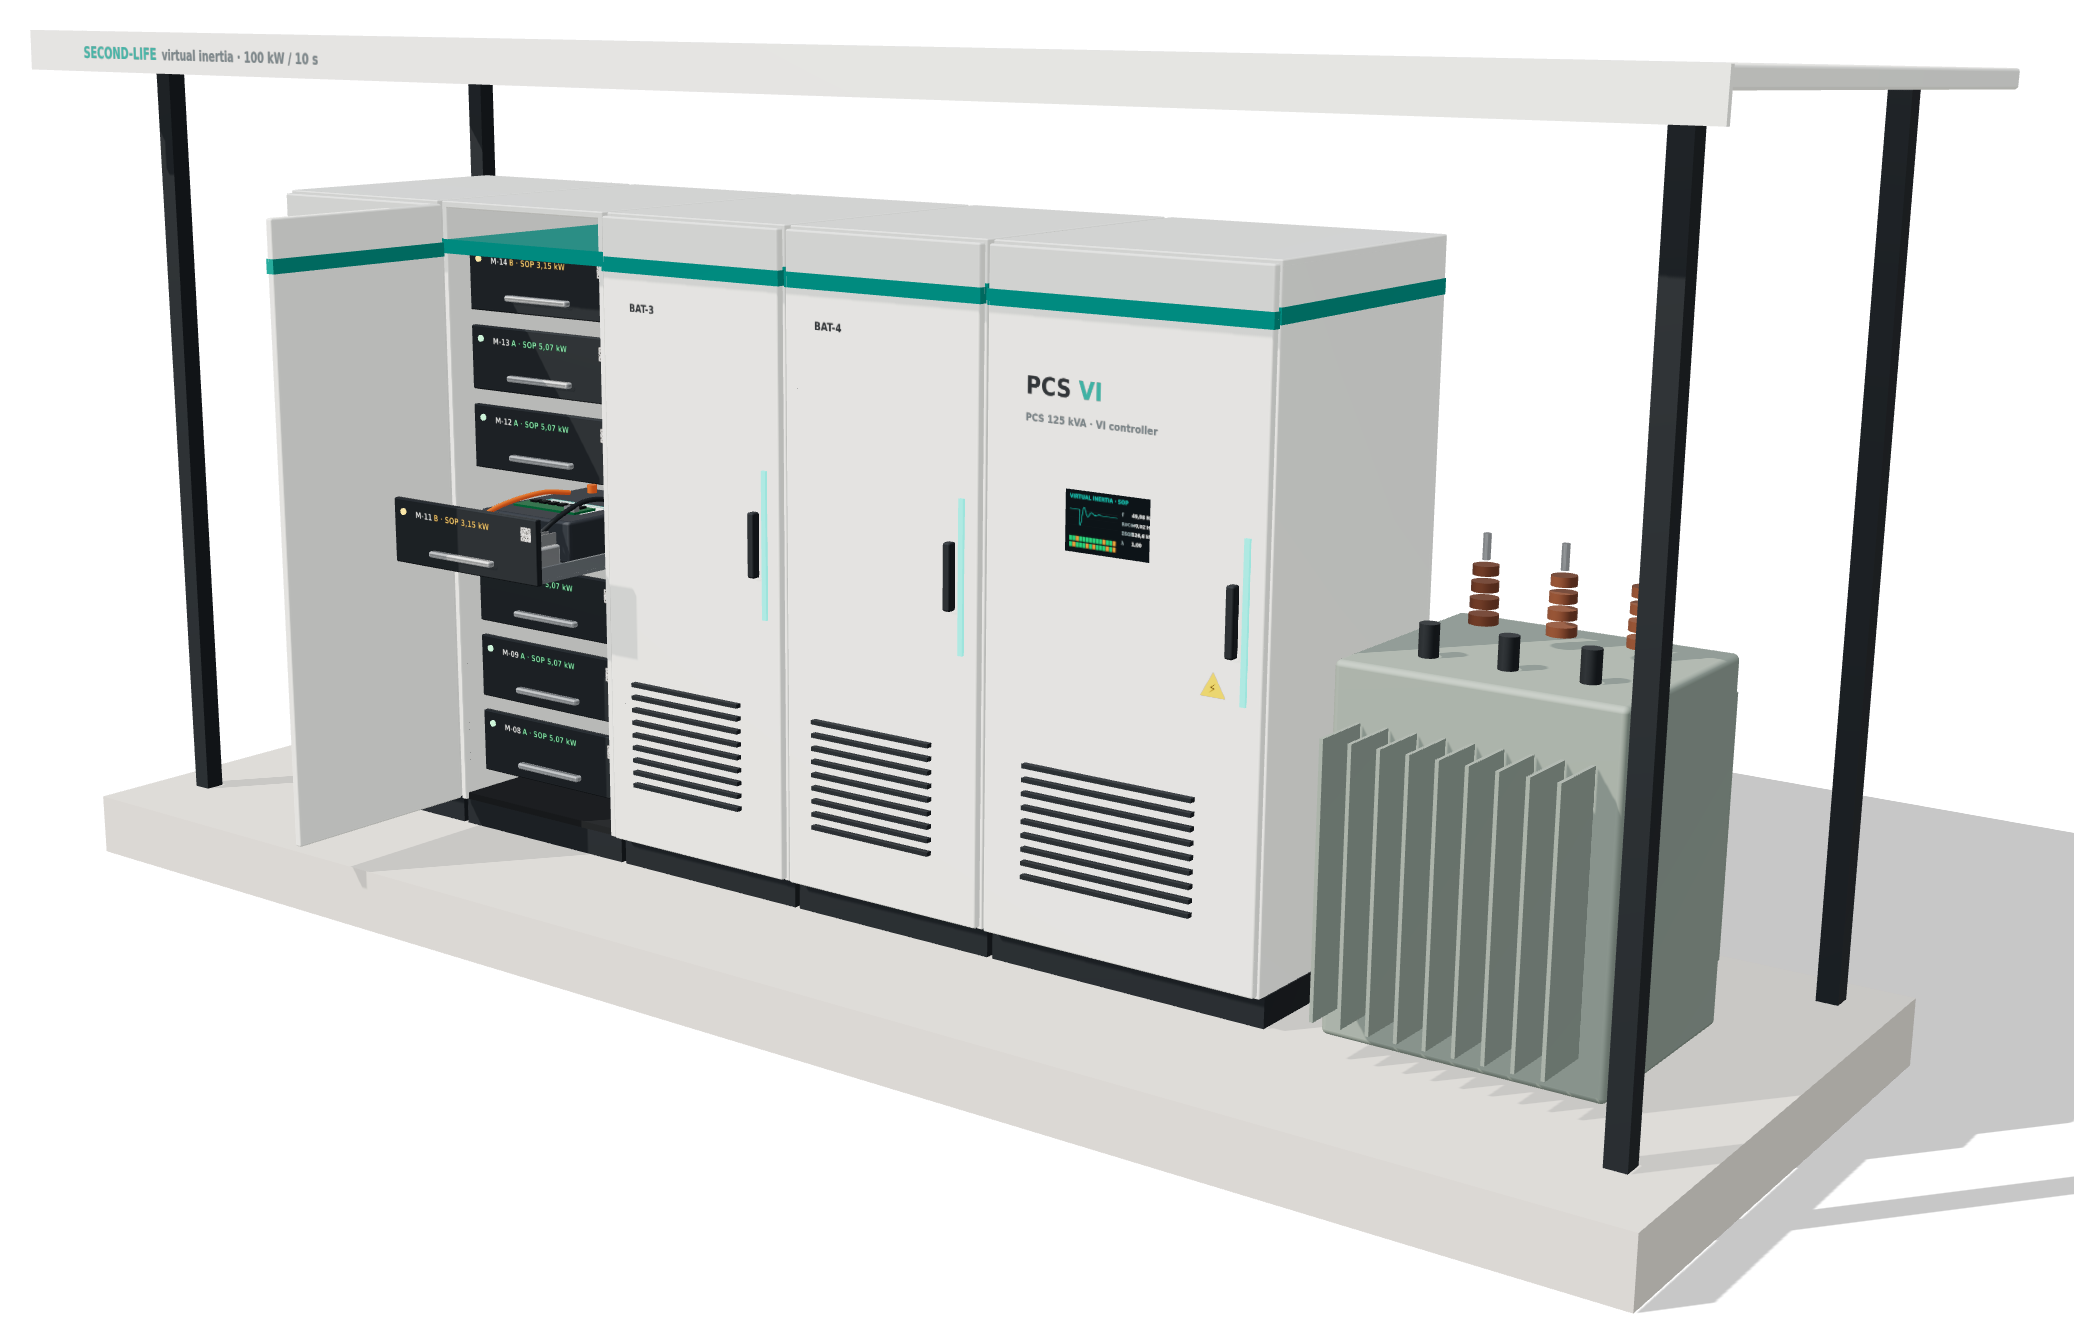
\includegraphics[width=\linewidth]{../figures/render_hero.png}};
\begin{scope}[x={(img.south east)},y={(img.north west)}]
\lead{0.1858}{0.6327}{0.06}{0.40}{north west}{Laci modul\\ditarik dari depan}
\lead{0.3609}{0.492}{0.30}{0.10}{north}{4 kabinet baterai, 7 laci per kabinet}
\lead{0.5401}{0.6816}{0.60}{0.98}{south}{Kabinet PCS: inverter 125 kVA\\dan pengendali VI}
\lead{0.7065}{0.4453}{0.78}{0.12}{north}{Trafo 0,4/20 kV}
\lead{0.1336}{0.9634}{0.30}{1.02}{south west}{Atap peneduh}
\end{scope}
\end{tikzpicture}
\end{minipage}

\vfill
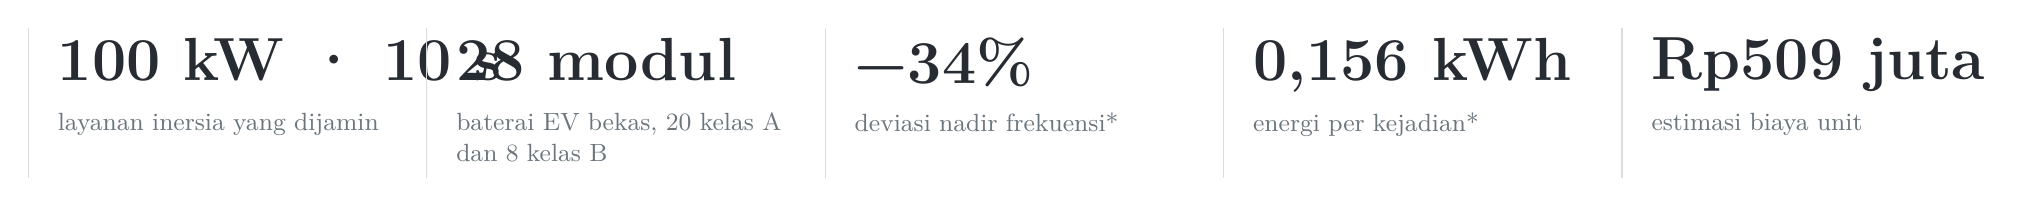
\begin{tikzpicture}
\def\w{5.06}
\foreach \i/\bg/\sm in {0/{100 kW · 10 s}/{layanan inersia yang dijamin},1/{28 modul}/{baterai EV bekas, 20 kelas A dan 8 kelas B},2/{−34\%}/{deviasi nadir frekuensi*},3/{0,156 kWh}/{energi per kejadian*},4/{Rp509 juta}/{estimasi biaya unit}}{
  \draw[hair,line width=0.5pt] (\i*\w+0.0,0) -- (\i*\w+0.0,1.9);
  \node[anchor=north west,font=\fontsize{22}{22}\selectfont\bfseries,text=ink] at (\i*\w+0.25,1.9) {\bg};
  \node[anchor=north west,font=\small,text=mute,text width=4.5cm] at (\i*\w+0.25,0.95) {\sm};
}
\end{tikzpicture}\\[2pt]
{\footnotesize\color{mute} *Simulasi representatif gangguan 250 kW pada sistem diesel 3 MVA, H = 1,5 s; bukan data lapangan PLN.}

\newpage
%% ---------------- Halaman 2: laci ----------------
\header{Laci modul}{2}
\vspace*{0.2cm}
{\LARGE\bfseries Satu modul, satu laci}\\[4pt]
{\normalsize\color{mute} Modul bekas tidak seragam. Karena setiap laci punya BMS dan DC/DC sendiri, modul lemah cukup diberi beban lebih kecil atau dilepas tanpa mematikan unit.}\\[0.5cm]
\begin{minipage}[t]{0.57\linewidth}
\centering
\begin{tikzpicture}
\node[anchor=south west,inner sep=0] (img) at (0,0) {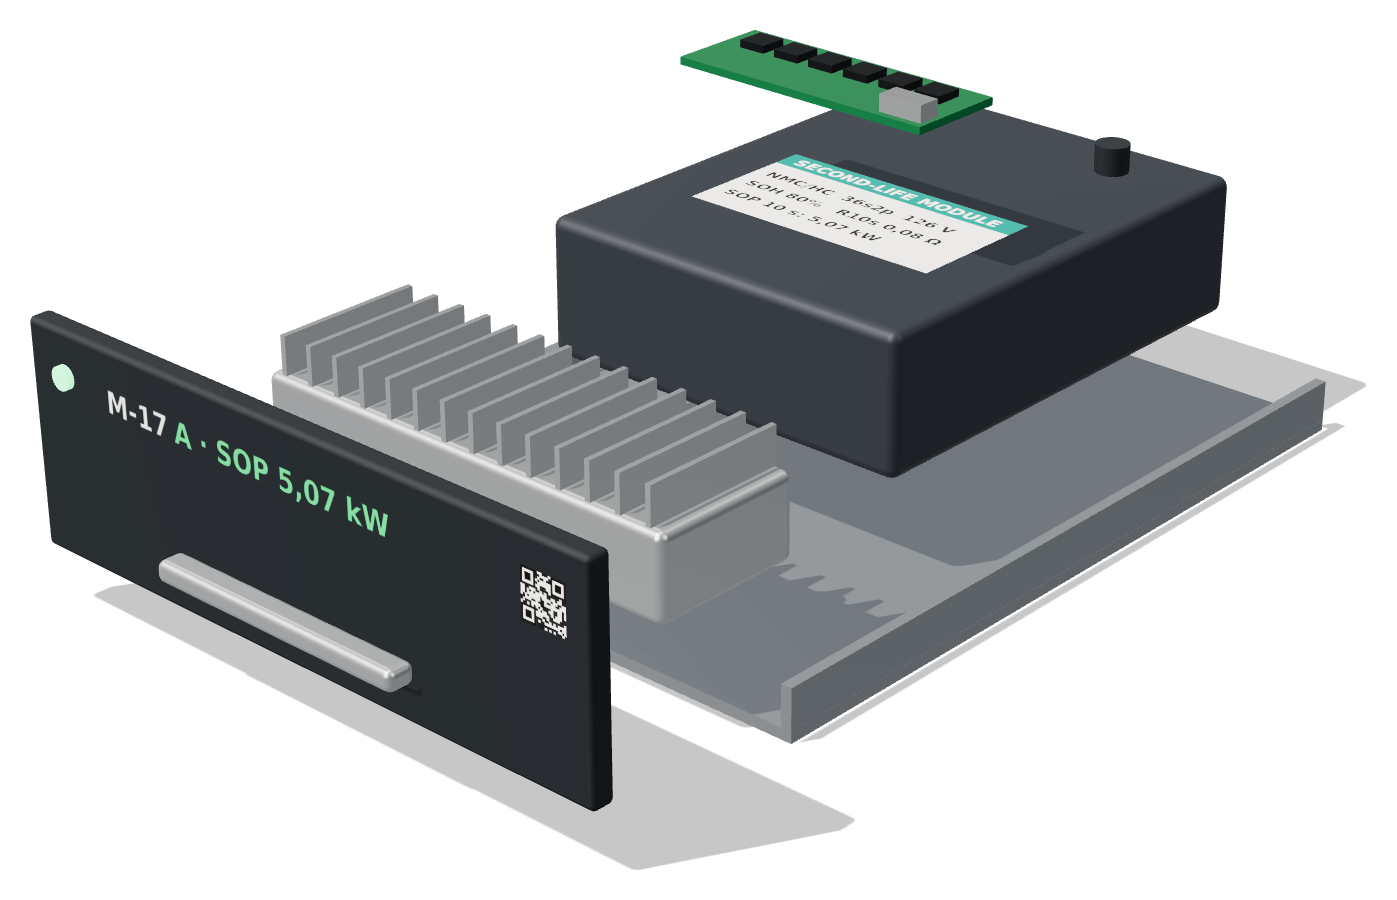
\includegraphics[width=0.95\linewidth]{../figures/render_drawer.png}};
\begin{scope}[x={(img.south east)},y={(img.north west)}]
\callout{0.86}{0.70}{1}
\callout{0.70}{0.94}{2}
\callout{0.50}{0.62}{3}
\callout{0.06}{0.66}{4}
\callout{0.40}{0.24}{5}
\callout{0.93}{0.45}{6}
\end{scope}
\end{tikzpicture}\\[6pt]
\small
\begin{tabular}{@{}l p{6.3cm} l p{6.3cm}@{}}
\num{1} & \textbf{Modul EV bekas} NMC/HC 36s2p, 126 V & \num{4} & \textbf{Panel depan}, LED hijau A / kuning B \\[3pt]
\num{2} & \textbf{BMS}: tegangan sel, arus, suhu & \num{5} & \textbf{QR SOP passport} \\[3pt]
\num{3} & \textbf{DC/DC dua arah terisolasi 6 kW} & \num{6} & \textbf{Nampan geser}, ganti dari depan \\
\end{tabular}
\end{minipage}\hfill
\begin{minipage}[t]{0.40\linewidth}
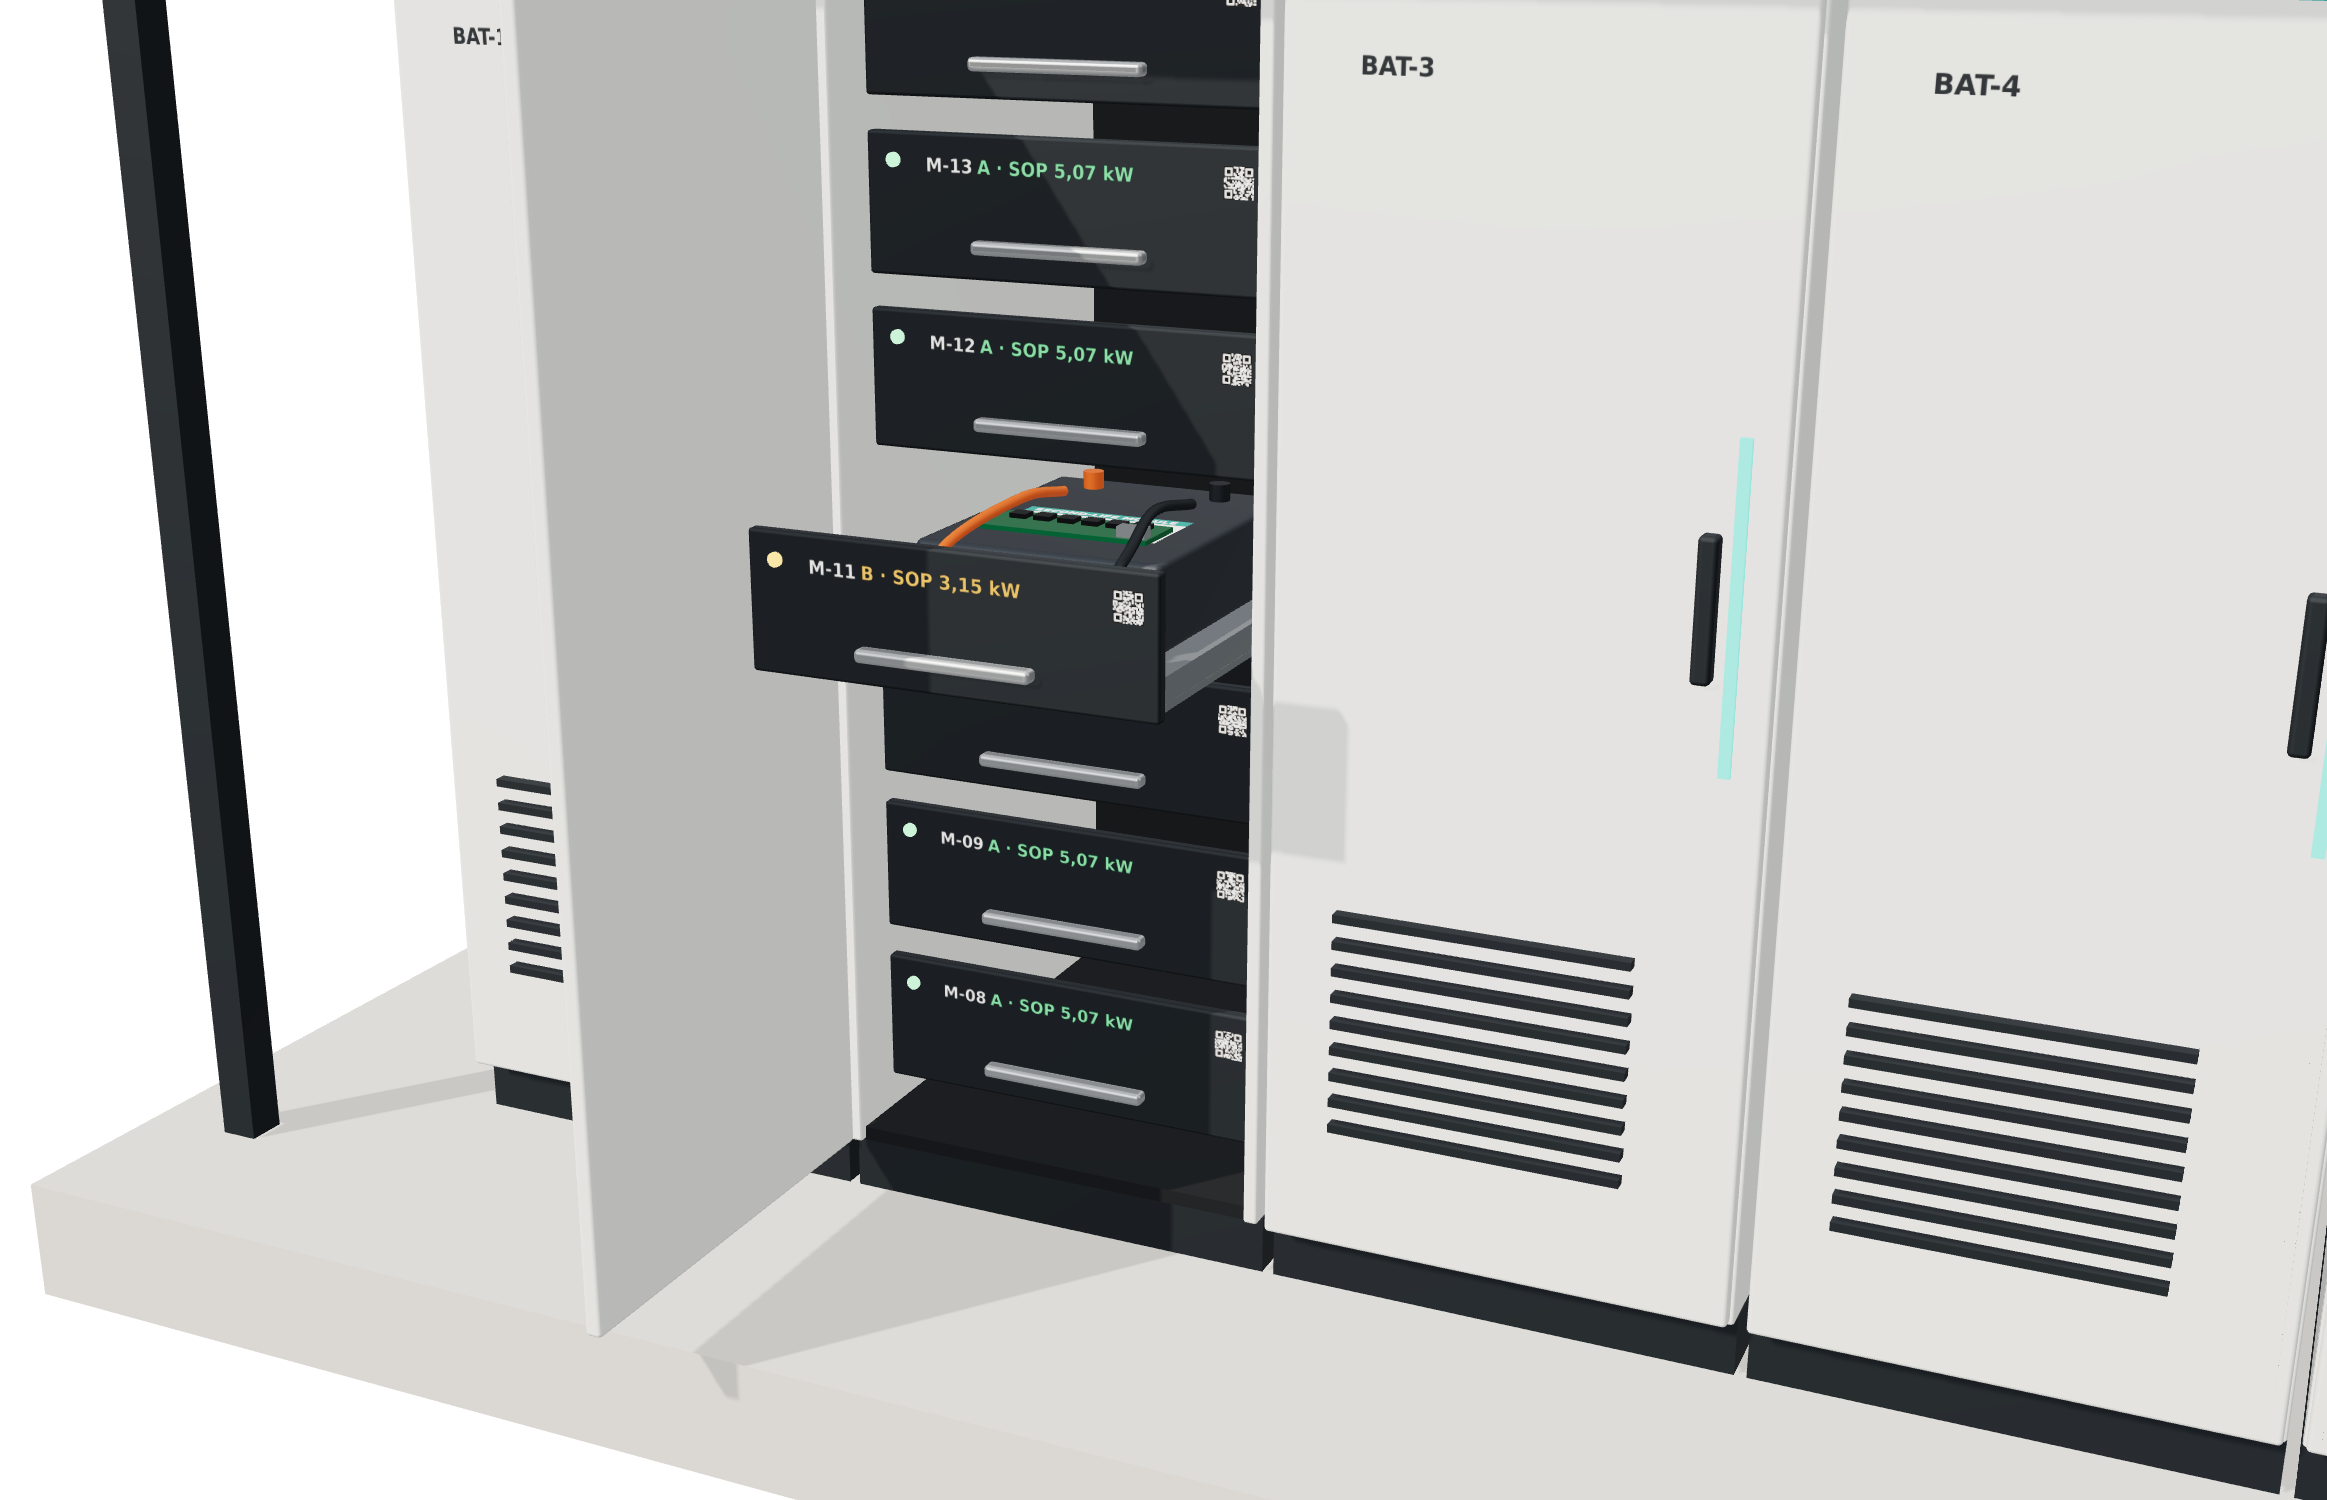
\includegraphics[width=\linewidth]{../figures/render_front.png}\\[4pt]
{\small\color{mute} Kabinet BAT-2 terbuka. Label di tiap laci menunjukkan nomor modul, kelas, dan SOP 10 detik.}\\[10pt]
\begin{tabular}{@{}p{3.3cm}p{2.0cm}p{2.0cm}@{}}
\toprule
\textbf{SOP passport} & \textbf{Kelas A} & \textbf{Kelas B} \\
\midrule
Jumlah modul & 20 & 8 \\
SOH kapasitas & 80\% & 70\% \\
$R_{10\,\mathrm{s}}$ & 0,08 Ω & 0,16 Ω \\
Batas arus & 40 A & 25 A \\
SOP 10 s & 5,07 kW & 3,15 kW \\
Beban saat 100 kW & 4,34 kW & 2,70 kW \\
\bottomrule
\end{tabular}
\end{minipage}

\newpage
%% ---------------- Halaman 3: eksterior dan dimensi ----------------
\header{Eksterior dan spesifikasi}{3}
\vspace*{0.2cm}
{\LARGE\bfseries Kabinet outdoor modular untuk lokasi pesisir}\\[4pt]
{\normalsize\color{mute} Kapasitas ditambah per kabinet. Atap peneduh mengurangi beban pendingin, pad beton menjaga unit dari genangan.}\\[0.4cm]
\begin{minipage}[c]{0.57\linewidth}
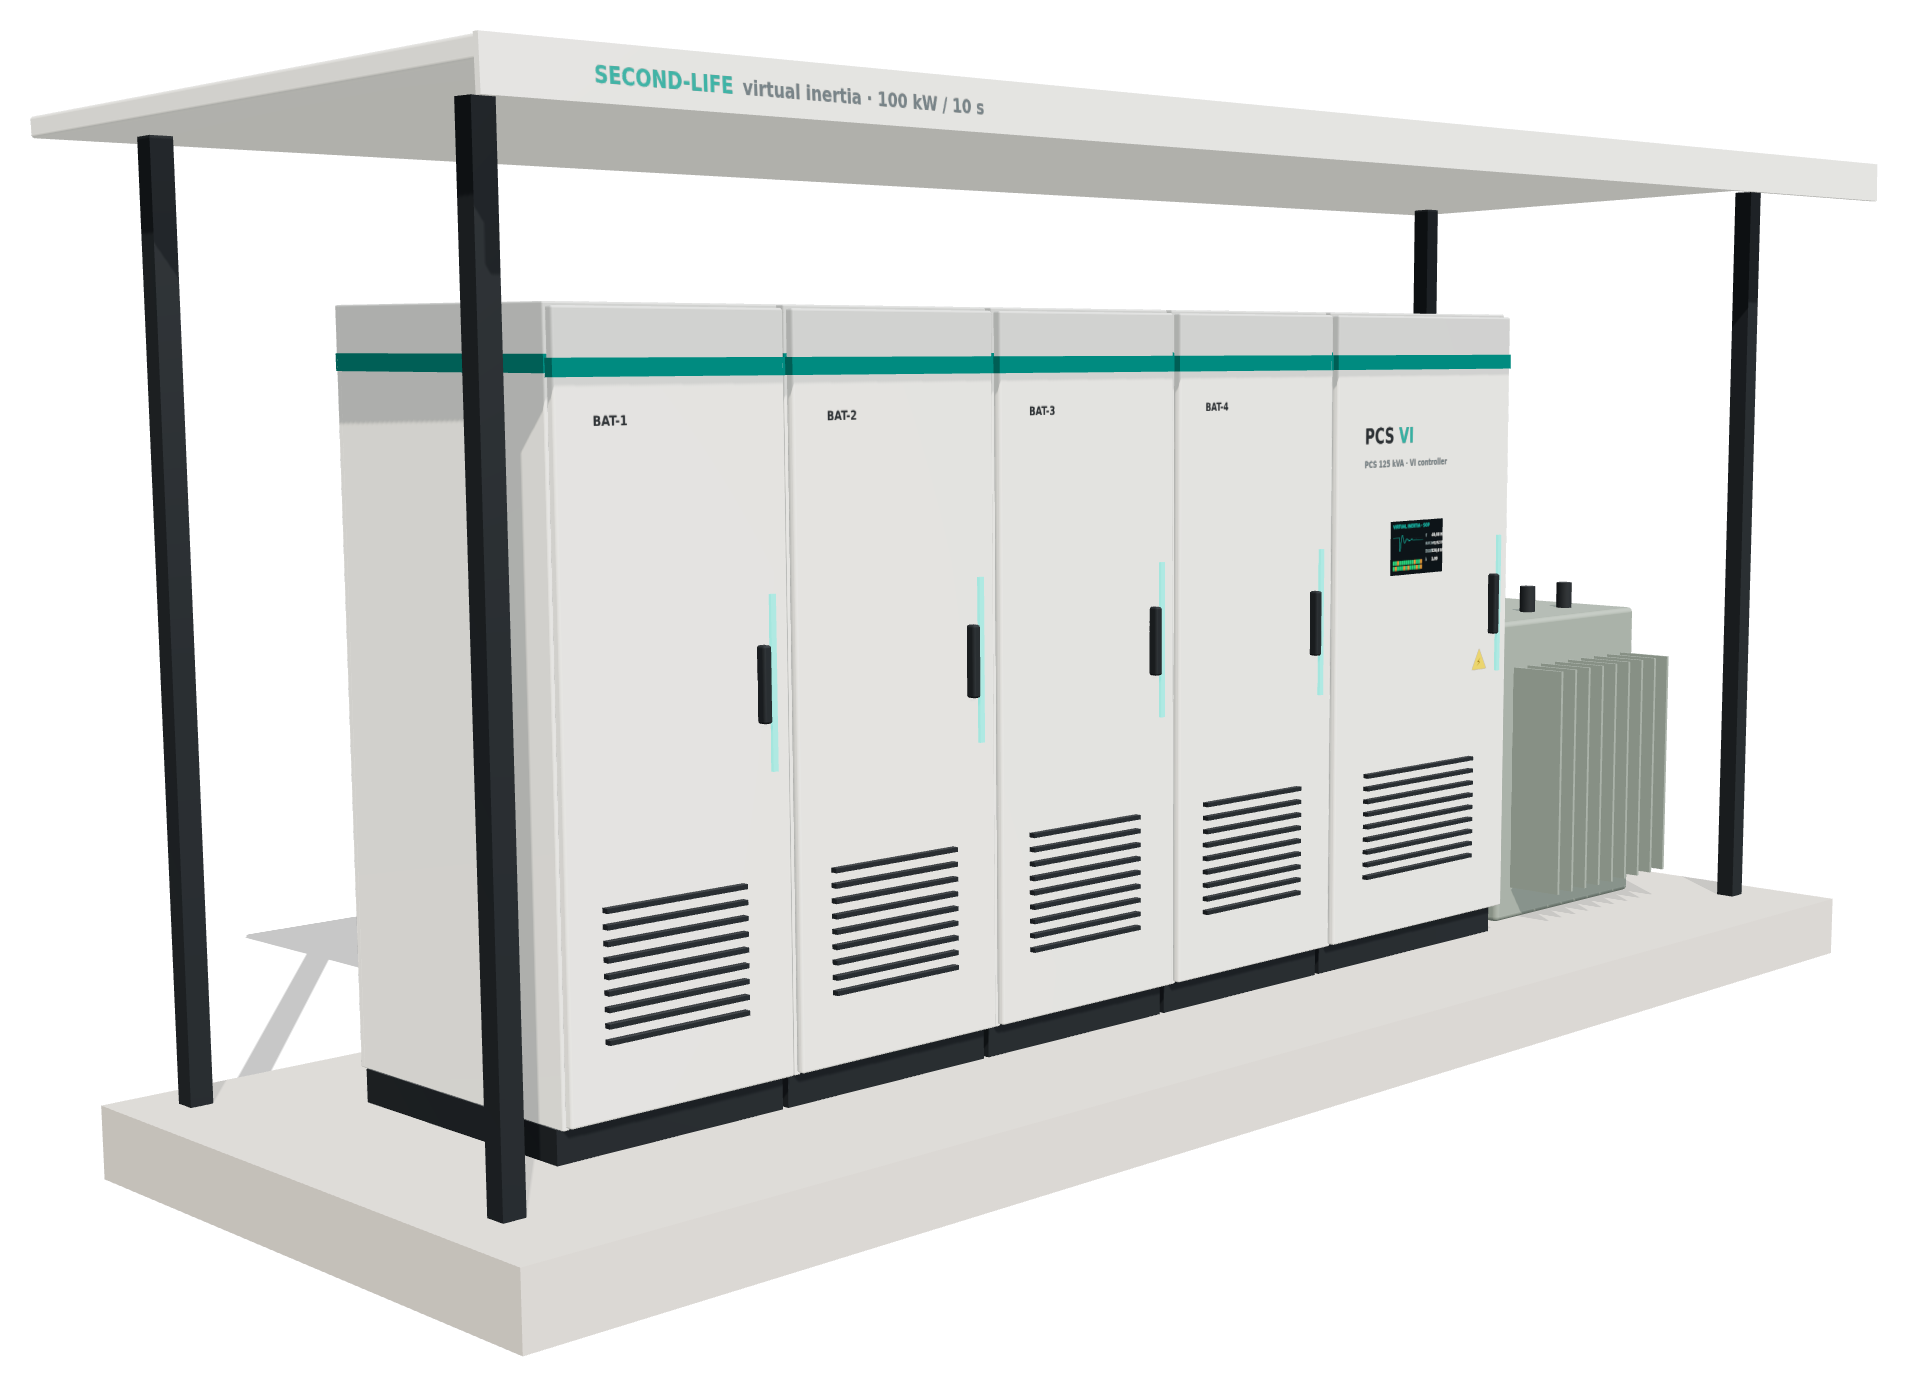
\includegraphics[width=\linewidth]{../figures/render_closed.png}
\end{minipage}\hfill
\begin{minipage}[c]{0.40\linewidth}
\small
\begin{tabular}{@{}p{3.6cm}p{6.0cm}@{}}
\toprule
\multicolumn{2}{@{}l}{\textbf{Spesifikasi rancangan}} \\
\midrule
Layanan & 100 kW selama 10 s, respons target $\le$ 100 ms \\
Modul & 28 × NMC/HC 36s2p bekas, energi efektif $\approx$ 85,7 kWh \\
Konverter modul & 28 × DC/DC dua arah terisolasi 6 kW \\
Bus DC & 750 V \\
Inverter & 3 fase, 125 kVA, \textit{grid-following} \\
Interkoneksi & trafo 0,4/20 kV ke titik sambung PLN \\
Kendali & $P=-\lambda K_v\,df/dt-\lambda K_d\,\Delta f$, \newline $K_v=80$ kW·s/Hz, $K_d=300$ kW/Hz \\
Pembagian daya & sebanding SOP tiap modul, dengan redistribusi \\
\midrule
\multicolumn{2}{@{}l}{\textbf{Dimensi perkiraan}} \\
\midrule
Kabinet baterai & 0,78 × 1,0 × 2,3 m (L × D × T), 4 unit \\
Kabinet PCS & 1,0 × 1,0 × 2,3 m \\
Deret kabinet & $\approx$ 4,2 m \\
Pad beton & 6,2 × 2,1 m \\
Tinggi atap peneduh & $\approx$ 3,0 m \\
\bottomrule
\end{tabular}
\end{minipage}

\newpage
%% ---------------- Halaman 4: cara kerja ----------------
\header{Cara kerja}{4}
\vspace*{0.2cm}
{\LARGE\bfseries Dari modul bekas ke inersia virtual}\\[0.6cm]
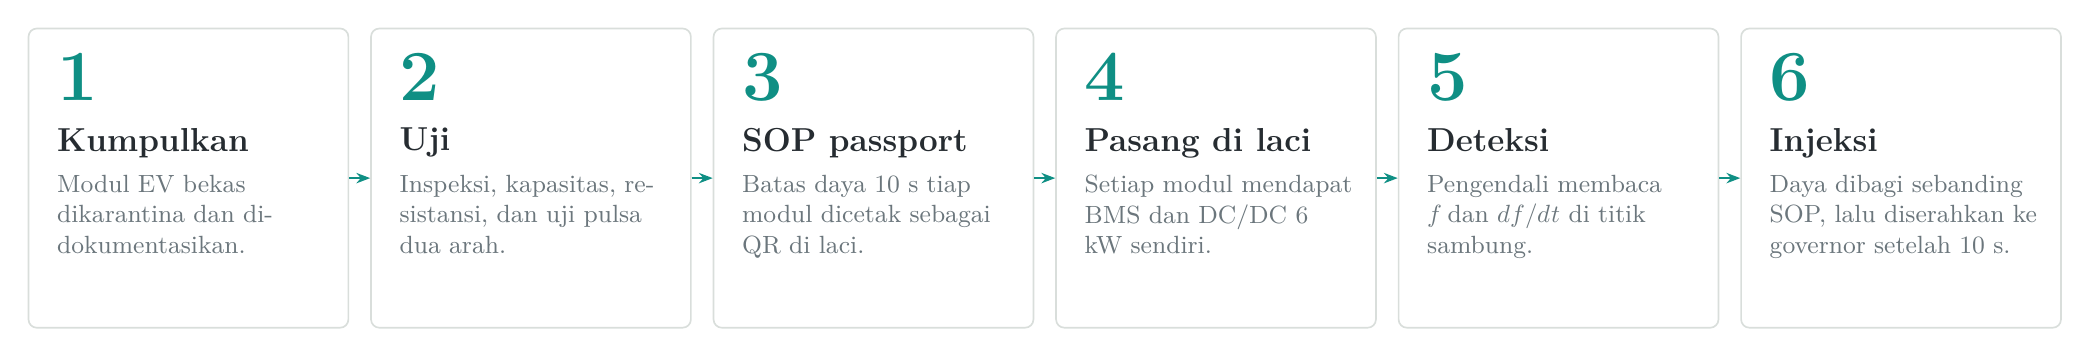
\begin{tikzpicture}[
  card/.style={draw=hair, line width=0.6pt, rounded corners=3pt, fill=white, minimum width=3.9cm, minimum height=3.8cm, align=left, anchor=north west, inner sep=8pt, text width=3.5cm},
  >={Stealth[length=5pt]}]
\foreach \i/\t/\d in {
  1/{Kumpulkan}/{Modul EV bekas dikarantina dan didokumentasikan.},
  2/{Uji}/{Inspeksi, kapasitas, resistansi, dan uji pulsa dua arah.},
  3/{SOP passport}/{Batas daya 10 s tiap modul dicetak sebagai QR di laci.},
  4/{Pasang di laci}/{Setiap modul mendapat BMS dan DC/DC 6 kW sendiri.},
  5/{Deteksi}/{Pengendali membaca $f$ dan $df/dt$ di titik sambung.},
  6/{Injeksi}/{Daya dibagi sebanding SOP, lalu diserahkan ke governor setelah 10 s.}}{
  \node[card] (s\i) at ({(\i-1)*4.35},0) {};
  \node[anchor=north west,font=\fontsize{26}{26}\selectfont\bfseries,text=teal] at ($(s\i.north west)+(0.25,-0.2)$) {\i};
  \node[anchor=north west,font=\large\bfseries,text=ink] at ($(s\i.north west)+(0.25,-1.15)$) {\t};
  \node[anchor=north west,font=\small,text=mute,text width=3.4cm,align=left] at ($(s\i.north west)+(0.25,-1.75)$) {\d};
}
\foreach \i [evaluate=\i as \j using int(\i+1)] in {1,...,5} \draw[->,teal,line width=0.8pt] (s\i.east) -- (s\j.west);
\end{tikzpicture}

\vfill
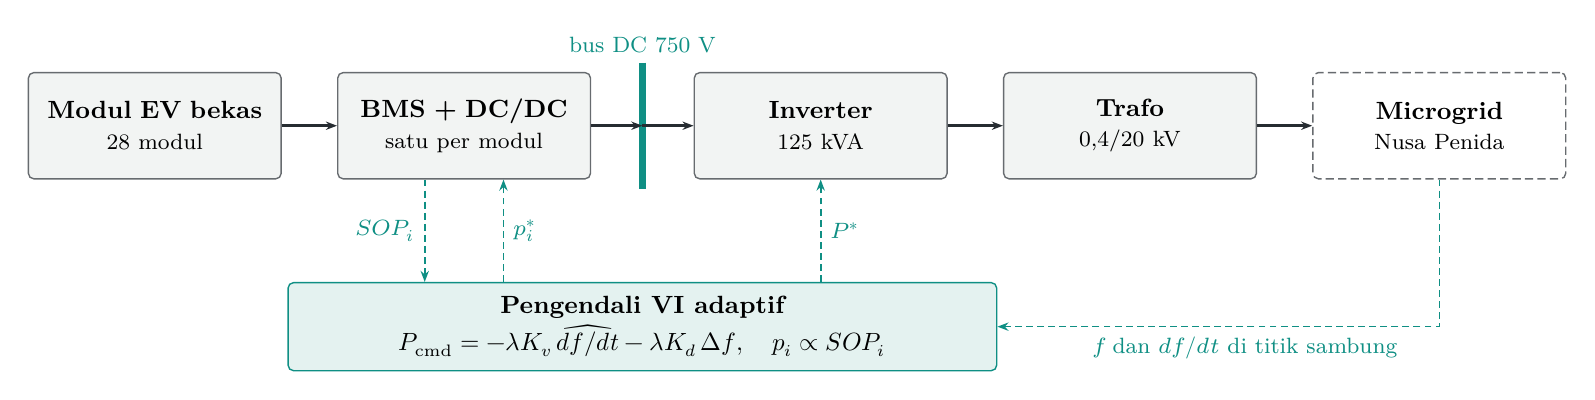
\begin{tikzpicture}[
  font=\small, >={Stealth[length=4pt]},
  blk/.style={draw=ink!70, line width=0.5pt, rounded corners=2pt, fill=soft, align=center, minimum height=1.35cm, text width=3.0cm, inner sep=3pt},
  pw/.style={->, draw=ink, line width=0.9pt},
  sg/.style={->, draw=teal, line width=0.6pt, dash pattern=on 2.5pt off 1.5pt},
  lbl/.style={font=\footnotesize, text=teal}]
\node[blk] (mod) {\textbf{Modul EV bekas}\\{\footnotesize 28 modul}};
\node[blk, right=0.7cm of mod] (dc) {\textbf{BMS + DC/DC}\\{\footnotesize satu per modul}};
\coordinate (busx) at ($(dc.east)+(0.65,0)$);
\draw[teal, line width=2.6pt] ($(busx)+(0,0.8)$) -- ($(busx)+(0,-0.8)$);
\node[font=\footnotesize, text=teal, above] at ($(busx)+(0,0.8)$) {bus DC 750 V};
\node[blk, right=1.3cm of dc] (inv) {\textbf{Inverter}\\{\footnotesize 125 kVA}};
\node[blk, right=0.7cm of inv] (tr) {\textbf{Trafo}\\{\footnotesize 0,4/20 kV}};
\node[blk, right=0.7cm of tr, fill=white, dash pattern=on 3pt off 1.5pt] (mg) {\textbf{Microgrid}\\{\footnotesize Nusa Penida}};
\draw[pw] (mod) -- (dc); \draw[pw] (dc.east) -- (busx); \draw[pw] (busx) -- (inv.west);
\draw[pw] (inv) -- (tr); \draw[pw] (tr) -- (mg);
\node[draw=teal, fill=tealsoft, line width=0.5pt, rounded corners=2pt, align=center, inner sep=5pt,
      minimum height=1.1cm, minimum width=9cm, anchor=north] (ctl) at ($(dc.south)!0.5!(inv.south)+(0,-1.3)$)
  {\textbf{Pengendali VI adaptif}\\[1pt] $P_{\mathrm{cmd}}=-\lambda K_v\,\widehat{df/dt}-\lambda K_d\,\Delta f,\quad p_i\propto SOP_i$};
\coordinate (s1) at ($(dc.south)+(-0.5,0)$); \coordinate (s2) at ($(dc.south)+(0.5,0)$);
\draw[sg] (s1) -- node[lbl, left] {$SOP_i$} (s1 |- ctl.north);
\draw[sg] (s2 |- ctl.north) -- node[lbl, right] {$p_i^{*}$} (s2);
\draw[sg] (inv.south |- ctl.north) -- node[lbl, right] {$P^{*}$} (inv.south);
\draw[sg] (mg.south) |- node[lbl, pos=0.72, below] {$f$ dan $df/dt$ di titik sambung} (ctl.east);
\end{tikzpicture}
\vfill
\end{document}
